\subsection {Session 5, Exercise 2}

\lineparagraph {Exercise}

Let the transition function of the 1-tape Turing-machine be

\begin{align*}
    \delta(q_0,1) = (q_1,1,R)\\
    \delta(q_0,*) = (q_2,*,R)\\
    \delta(q_1,1) = (q_3,1,R)\\
    \delta(q_3,1) = (q_0,1,R)
\end{align*}


start state is $q_0$, accept state is $q_3$. What is the language recognized by this machine?

\lineparagraph {Solution}

It's easier to see what's happening if we draw the machine:

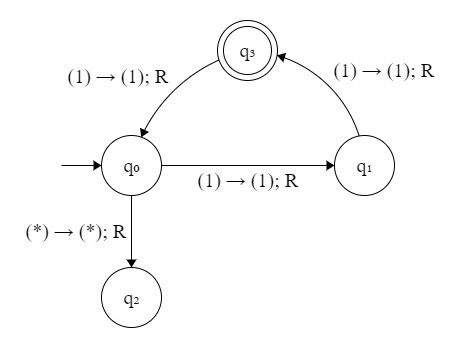
\includegraphics[width=0.5\linewidth]{05/6_2.png}

It the $q_0, q_1, q_3$ cycle reads the input word on the tape from left to right and counts the number of $1$'s modulo $3$. In $q_0$ the remainder is $0$, in $q_1$ the remainder is $1$ and in $q_3$ the remainder is $2$.

When the input is $\varepsilon$ (the empty string) the $q_0 \xrightarrow{(*) \rightarrow (*);\text{ }R} q_2$ transition will move the machine to $q_2$ and it will halt there, since there is no transitions defined, thus reject the empty string input. (This transition could have been left out, since then the machine would remain in $q_0$ and reject the empty string input similarly.)

Since the accept state is $q_3$, words containing $3k+2$ number of $1$'s will be accepted, where $k\geq{}0$.

Notice how the above Turing-machine does exactly the same thing as this Finite Automaton:

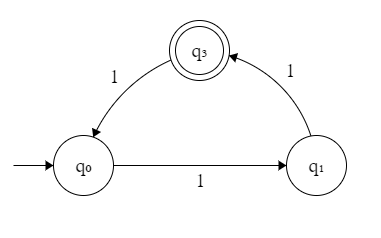
\includegraphics[width=0.6\linewidth]{05/6_2_b.png}

We have seen similar modulo counter automatons on the first practice session.